\chapter{BaseLib Level 6}
\chaptermark{Level 6}


INTRO TODO


\begin{itemize}
 \item Memory Mapped CDB
 \item Mathematic support library
 \item HTTP Browsing
 \item System Support
\end{itemize}




\section{Memory Mapped CDB}

TODO INTRO

TODO logical schema

\begin{figure}[h!]
 \begin{center}
  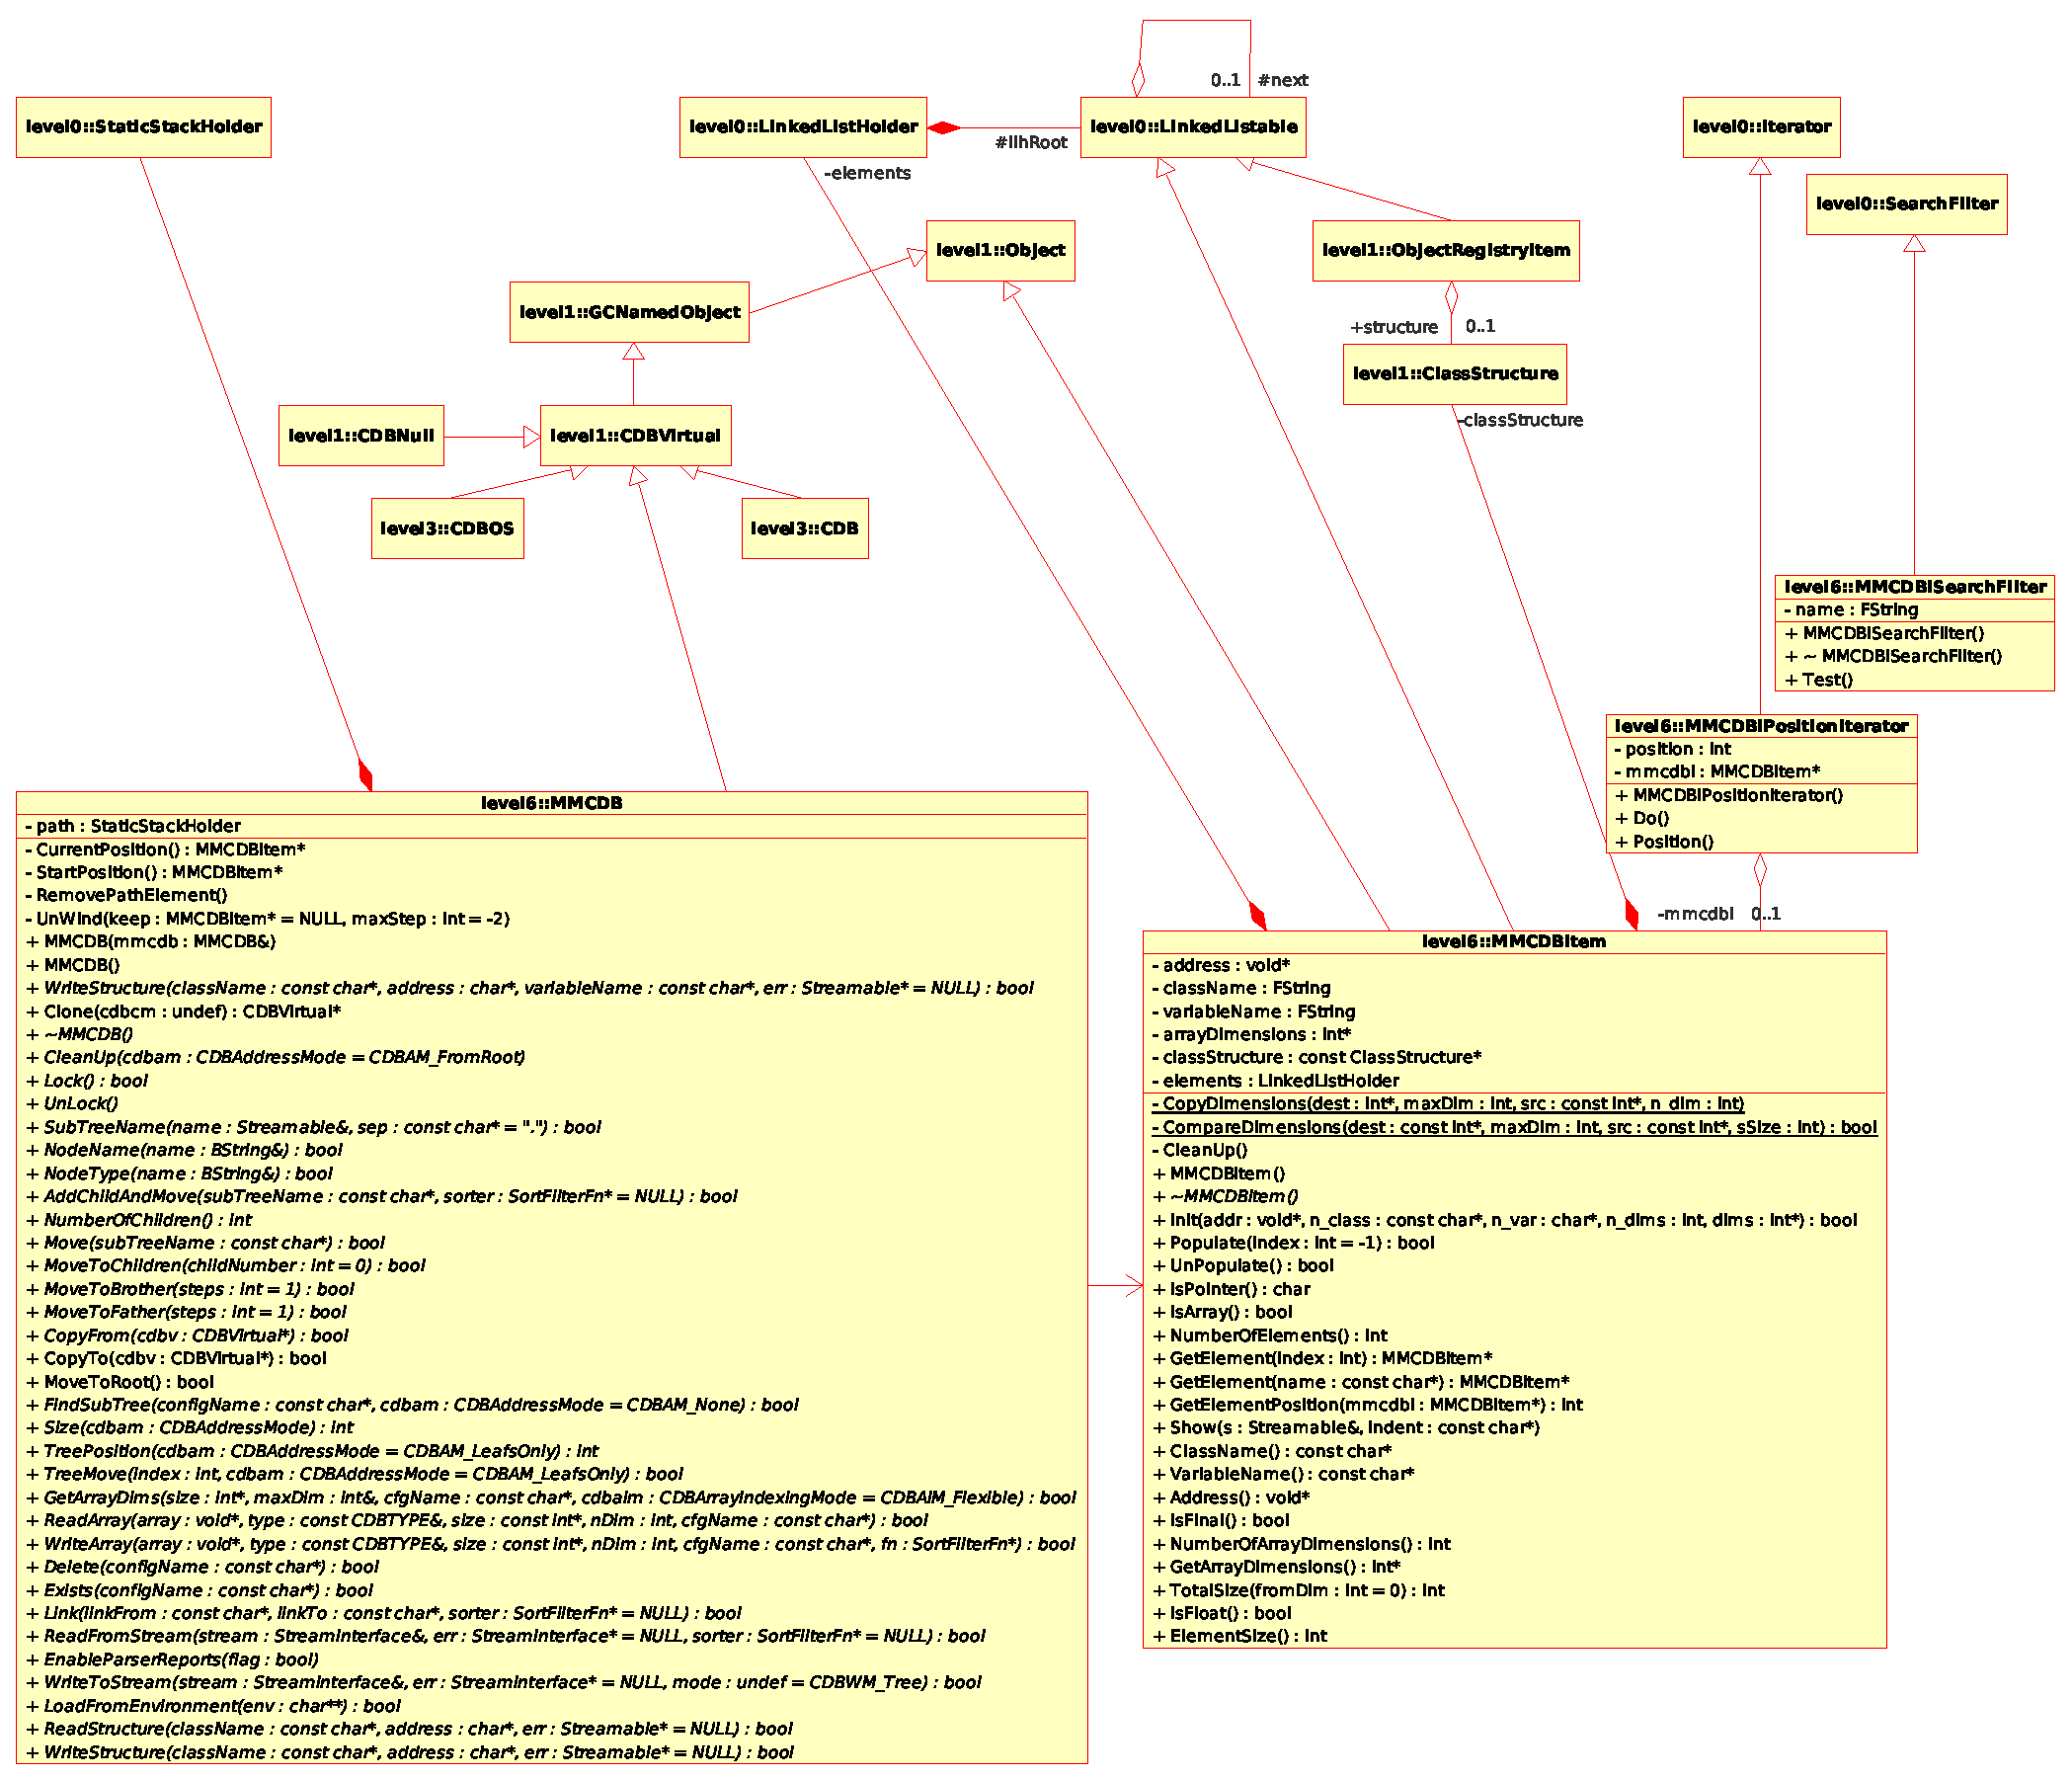
\includegraphics[width=1.1\textwidth]{level6/level6-MMCDB-exp.eps}
  \caption{BaseLib Level 6 Memory Mapped CDB}
  \label{f:level6:MMCDB}
 \end{center}
\end{figure}

\begin{itemize}
 \item MMCDBItem, MMCDBISearchFilter, MMCDBIPositionIterator
 \item MMCDB
\end{itemize}



\subsubsection{MMCDBItem}
\texttt{[MMCDBItem.h, MMCDBItem.cpp]}\\
An \texttt{MMCDBItem} is used by an MMCDB object as elements of a path. It is a contianer of elements of the same type. It inherits from \texttt{LinkedListable} and \texttt{Object}. \\


Attributes are not setted by the constructor by the \texttt{Init} method, only the attribute \texttt{elements} is setted up by the \texttt{Populate} method. The attribute \texttt{address} is the address of the variable, \texttt{className} stores the class name of the variable and the \texttt{variableName} the name of the variable itself; \texttt{arrayDimensions} is a NULL terminated list of dimensions, \texttt{classStructure} is a class structure associated to the class. The last attribute is a \texttt{LinkedListHolder} that is the one loaded by the \texttt{Populate} method.

\begin{lstlisting}[
extendedchars=true,%
basicstyle=\fontfamily{pcr}\fontseries{m}\selectfont\footnotesize, %
stepnumber=1,%
numberstyle=\tiny,%
keywordstyle=\footnotesize\tt ,%
language=C++]
private:
   void* address;
   FString className;
   FString variableName;
   int* arrayDimensions;
   const ClassStructure* classStructure;

private:
   LinkedListHolder elements;
\end{lstlisting}

The list of methods starts with two static methods; \texttt{CopyDimensions} copies all the dimensions that fit and collapses the last, \texttt{CompareDimensions} simply compare the \texttt{arrayDimensions}, but the arrays must be the same or comaptible. \texttt{CleanUp} deallocates memory. \\

The method \texttt{Init} initializes attributes, the last three parameters are only necessary to handle packed structures. The method \texttt{Populate} set up the linked list, in case of a structure creates virtaul view of the structure, in case of an arry does nothing and if (\texttt{index} its greater then zero) then it will populate one array row; \texttt{UnPopulate} basically de-populate elements. \\


The method \texttt{IsPointer} return \texttt{True} whether this is a pointer or not; the same can be said for \texttt{IsArray}. \texttt{IsFloat} is used for elementary types to know whether this is a \texttt{float} or \texttt{double}.

\begin{lstlisting}[
extendedchars=true,%
basicstyle=\fontfamily{pcr}\fontseries{m}\selectfont\footnotesize, %
stepnumber=1,%
numberstyle=\tiny,%
keywordstyle=\footnotesize\tt ,%
language=C++]
   static void CopyDimensions(int* destination,int maxDim,const int* source,
      int numberOfDimensions);
   static bool CompareDimensions(const int* destination,int maxDim,const int* source,
      int sSize);

   void CleanUp();
public:
   MMCDBItem();
   virtual ~MMCDBItem();

   bool Init(void* address,const char* className,const char* variableName,
      int numberOfDimensions=0,int* dimensions=NULL);

   bool Populate(int index=-1);
   bool UnPopulate();

   bool IsPointer();
   bool IsArray();
   bool IsFloat();

   int NumberOfElements();

   MMCDBItem* GetElement(int index);
   MMCDBItem* GetElement(const char* name);
   int GetElementPosition(MMCDBItem* mmcdbi);

   void Show(Streamable& s,const char* indent);
   const char* ClassName() const;
   const char* VariableName() const;
   void* Address() const;

   bool IsFinal();
   int NumberOfArrayDimensions();
   int* GetArrayDimensions()

   int TotalSize(int fromDim=0);
   int ElementSize();
\end{lstlisting}



\subsubsection{MMCDBISearchFilter}
\texttt{[MMCDBItem.h]}\\
The class \texttt{MMCDBISearchFilter} serches members for a given name, it inherits as usual from \texttt{SearchFilter}. The single attribute \texttt{name} accounts for the name to search for. The method \texttt{Test} is that one that performs the search on a set of data.

\begin{lstlisting}[
extendedchars=true,%
basicstyle=\fontfamily{pcr}\fontseries{m}\selectfont\footnotesize, %
stepnumber=1,%
numberstyle=\tiny,%
keywordstyle=\footnotesize\tt ,%
language=C++]
   FString name;
public:
   MMCDBISearchFilter(const char* name);
   virtual ~MMCDBISearchFilter();

   virtual bool Test (LinkedListable* data);
\end{lstlisting}



\subsubsection{MMCDBIPositionIterator}
\texttt{[MMCDBItem.h, MMCDBItem.cpp]}\\
The class \texttt{MMCDBIPositionIterator} finds the node position, it inherits from \texttt{Iterator}; the attribute \texttt{mmcdbi} is the object to search for, it will be NULL after found.

\begin{lstlisting}[
extendedchars=true,%
basicstyle=\fontfamily{pcr}\fontseries{m}\selectfont\footnotesize, %
stepnumber=1,%
numberstyle=\tiny,%
keywordstyle=\footnotesize\tt ,%
language=C++]
   int position;
   MMCDBItem* mmcdbi;

public:
   MMCDBIPositionIterator(MMCDBItem* mmcdbi);

   virtual void Do (LinkedListable* data);
   int Position();
\end{lstlisting}



\subsubsection{MMCDB}
\texttt{[MMCDB.h, MMCDB.cpp}\\
The class \texttt{MMCDB} is a tool to access a block of memory as a CDB, the block of memory is described by a class or structure name, the name must be registered. An MMCDB is another kind of CDB that inherits from \texttt{CDBVirtual}. It defines only one attribute, \texttt{path}, of type \texttt{StaticStackHolder} (a dynamic vector that implements the standard stack push and pop operations). \\


The method \texttt{CurrentPosition} gets an \texttt{MMCDBItem} object pointer of the last path position; \texttt{StartPosition} gets the root path position; \texttt{RemovePathElement} removes the last path position, deallocation is performed only if this is the last left. The method \texttt{UnWind} removes all the path elements until the one specified in \texttt{maxStep}, if \texttt{maxStep} argument is below or equal $-2$ means to remove all elements if equal to $-1$ means leave father. \\


The method \texttt{WriteStructure} either copies or references a memory structure at address \texttt{address} and of type \texttt{className}, note that a CDB transforms the memory but a MMCDB just references it.
The method \texttt{Clone} creates a new reference to a database, or if that is not possible it creates a copy of it. \texttt{CleanUp} does nothing; \texttt{Lock} and \texttt{UnLock} doesn't block and simply return.

\begin{lstlisting}[
extendedchars=true,%
basicstyle=\fontfamily{pcr}\fontseries{m}\selectfont\footnotesize, %
stepnumber=1,%
numberstyle=\tiny,%
keywordstyle=\footnotesize\tt ,%
language=C++]
private:
   StaticStackHolder path;

   MMCDBItem* CurrentPosition();
   MMCDBItem* StartPosition();
   void RemovePathElement();
   void UnWind(MMCDBItem* keep=NULL,int maxStep=-2);

public:
   MMCDB(MMCDB &mmcdb);
   MMCDB();
   virtual ~MMCDB();

   virtual bool WriteStructure(const char* className,char* address,const char* variableName,
      Streamable* err=NULL);

   CDBVirtual* Clone(CDBCreationMode cdbcm);
   virtual void CleanUp(CDBAddressMode cdbam = CDBAM_FromRoot);

   virtual bool Lock();
   virtual void UnLock();
\end{lstlisting}

The method \texttt{SubTreeName} finds the overall path leading to the current node; the method \texttt{NodeName} returns in the \texttt{BString} argument the name of the current node, \texttt{NodeType} gets the type of the current node. The method \texttt{NumberOfChildren} returns how many branches from this node, negative numbers implies that the location is a leaf. \\


The method \texttt{AddChildAndMove} work as the following \texttt{Move} method; the method \texttt{Move} move to the specified location, the movement is relative to the current location. \texttt{MoveToChildren} move to a children, $0$ is the first of the childrens. \texttt{MoveToBrother} is similar and $0$ means remain where you are, greater then zero brothers on the right and below zero berothers on the left. \texttt{MoveToFather} lets you navigate to father and also to the root node; \texttt{MoveToRoot} moves back to the root calling \texttt{MoveToFather} with argument $-1$. \\


The method \texttt{CopyFrom} copies the pointed subtree in the \texttt{cdbv} into the current subtree. \texttt{CopyTo} copies the current subtree in the pointed \texttt{cdbv}. \\


The method \texttt{FindSubTree} searches on the right of the tree for the subtree identified by the string name, on success \texttt{nodes} attribute points to the node containing the subtree or leaf, it will not follow links.
The method \texttt{Size} returns the total number of nodes; \texttt{TreePosition} returns from left to right bottom to top order the absolute location of a node; \texttt{TreeMove} moves to a location within the whole (sub)tree; the nodes are numbered from left to right and from subnode to supernode; if the node does not exist returns \texttt{False} and remains in the start position. \\


The method \texttt{GetArrayDims} returns how many dimensions has the \texttt{MMCDBItem} returned by the \texttt{CurrentPosition} method. \texttt{ReadArray} and \texttt{WriteArray} read and write an array data structure in the \texttt{MMCDBItem} in the current position. \\


The method \texttt{Delete} will remove an entry or subtree (position is relative); to delete a link use the \texttt{linkTo} as the leaf name, to delete a subtree simply specify the group node; in this implementation \texttt{Delete} returns \texttt{False}. \texttt{Exists} return \texttt{True} if a certain entry exists. \texttt{Link} simply returns \texttt{False} and does nothing.

\begin{lstlisting}[
extendedchars=true,%
basicstyle=\fontfamily{pcr}\fontseries{m}\selectfont\footnotesize, %
stepnumber=1,%
numberstyle=\tiny,%
keywordstyle=\footnotesize\tt ,%
language=C++]
   virtual bool SubTreeName(Streamable& name,const char* sep = ".");
   virtual bool NodeName(BString& name);
   virtual bool NodeType(BString& name);
   virtual int NumberOfChildren();

   virtual bool AddChildAndMove(const char* subTreeName,SortFilterFn* sorter=NULL);
   virtual bool Move(const char* subTreeName);
   virtual bool MoveToChildren(int childNumber=0);
   virtual bool MoveToBrother(int steps=1);
   virtual bool MoveToFather(int steps=1);
   inline bool MoveToRoot();

   virtual bool CopyFrom(CDBVirtual* cdbv);
   inline bool CopyTo(CDBVirtual* cdbv);

   virtual bool FindSubTree(const char* configName,CDBAddressMode cdbam=CDBAM_None);
   virtual int Size(CDBAddressMode  cdbam);
   virtual int TreePosition(CDBAddressMode cdbam=CDBAM_LeafsOnly);
   virtual bool TreeMove(int index,CDBAddressMode cdbam=CDBAM_LeafsOnly);

   virtual bool GetArrayDims(int* size,int& maxDim,const char* configName,
      CDBArrayIndexingMode cdbaim=CDBAIM_Flexible);
   virtual bool ReadArray(void* array,const CDBTYPE& valueType,const int* size,
      int nDim,const char* configName);
   virtual bool WriteArray(const void* array,const CDBTYPE& valueType,const int* size,
      int nDim,const char* configName,SortFilterFn* sorter=NULL);

   virtual bool Delete(const char* configName);
   virtual bool Exists(const char* configName);
   virtual bool Link(const char* linkFrom,const char* linkTo,SortFilterFn* sorter=NULL);
\end{lstlisting}


Finally follow a set of complex load/save methods that are not implemented in this class and if they are functions return \texttt{False}.

Basically \texttt{ReadFromStream} should read a database from a stream; \texttt{EnableParserReports} enables reports of parser during \texttt{ReadFromStream} into \texttt{err} argument; \texttt{WriteToStream} writes the database to stream without any ordering; \texttt{LoadFromEnvironment} loads from environment or from any NULL terminated list of chars. \texttt{ReadStructure} will read a data structure from CDB to memory and \texttt{WriteStructure} will write a data structure from memory to CDB.

\begin{lstlisting}[
extendedchars=true,%
basicstyle=\fontfamily{pcr}\fontseries{m}\selectfont\footnotesize, %
stepnumber=1,%
numberstyle=\tiny,%
keywordstyle=\footnotesize\tt ,%
language=C++]
   virtual bool ReadFromStream(StreamInterface& stream,StreamInterface* err=NULL,
      SortFilterFn* sorter=NULL);
   virtual void EnableParserReports(bool flag);
   virtual bool WriteToStream(StreamInterface& stream,StreamInterface* err=NULL,
      CDBWriteMode mode=CDBWM_Tree);

   virtual bool LoadFromEnvironment(char** env);

   virtual bool ReadStructure(const char* className,char* address,
      Streamable* err=NULL);
   virtual bool WriteStructure(const char* className,char* address,
      Streamable* err=NULL);
\end{lstlisting}



\section{Mathematic Support Library}

\begin{figure}[h!]
 \begin{center}
  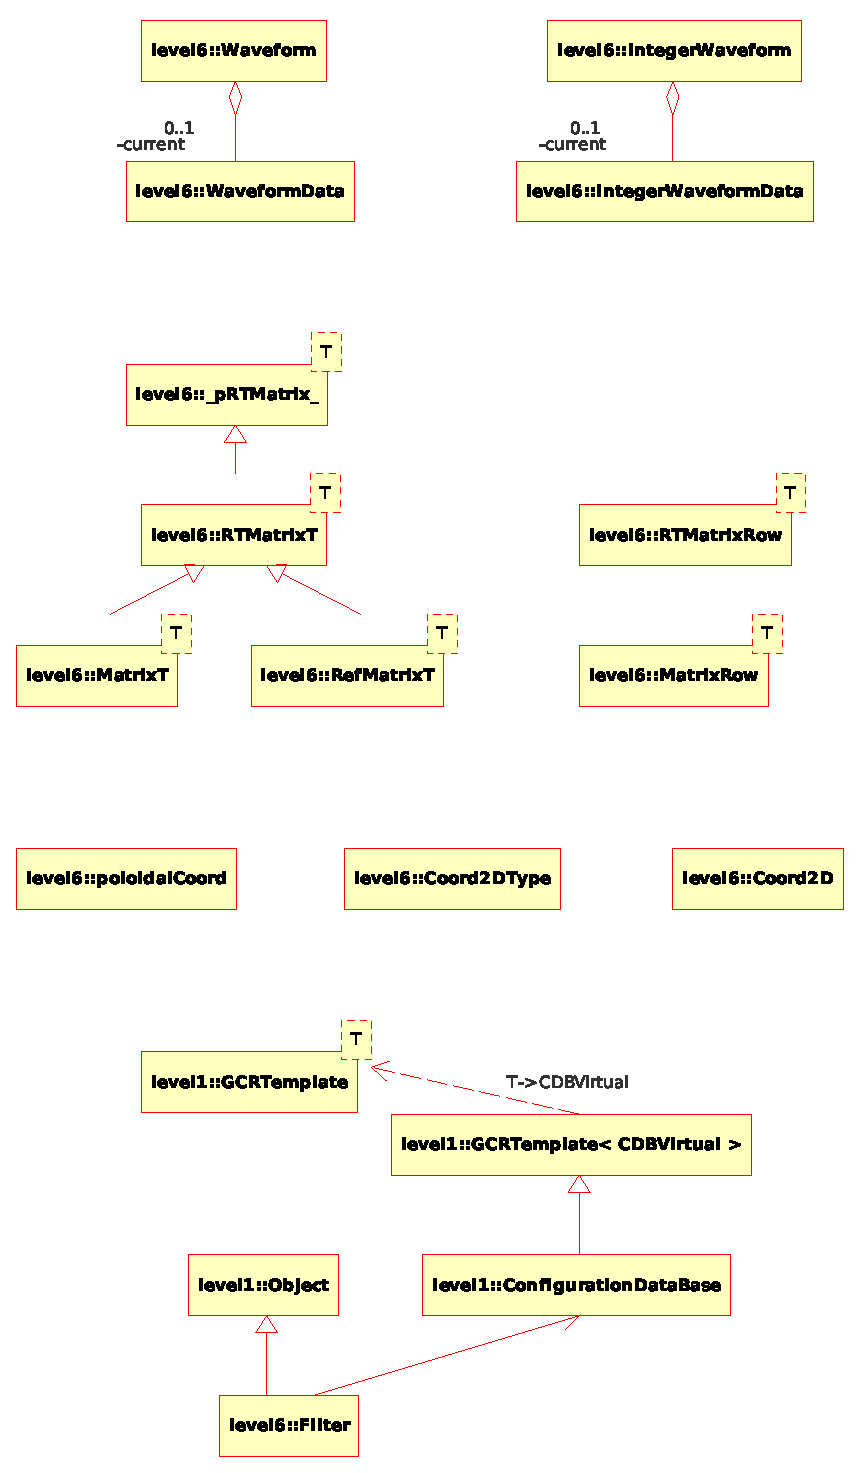
\includegraphics[width=0.53\textwidth]{level6/level6-math.eps}
  \caption{BaseLib Level 6 Mathematic Support Library}
  \label{f:level6:math}
 \end{center}
\end{figure}



\subsection{Matrix}

This section deal about matrix and matrix's operations. There are two main implementations: one with stringent bounds checks and another without boundary checks. The first is implemented with classes: \texttt{MatrixRow} and \texttt{MatrixT} and the other one with \texttt{RTMatrixRow} and \texttt{RTMatrixT}. The whole diagram is depicted in Figure \ref{f:level6:math-matrix}. \\

Classes with the name starting with \texttt{RT} are stripped from many methods and checks in boundary functions and so are more suitable to use it in real time (test it before using in Real Time). \\

Classes \texttt{MatrixRow} and \texttt{RTMatrixRow} implement a row matrix, \texttt{MatrixT} and \texttt{RTMatrixT} implement bidimensional matrix, no multidimensional matrix are currently implemented. \texttt{RefMatrixT} lets the user using a common C matrix.

\begin{figure}[h!]
 \begin{center}
  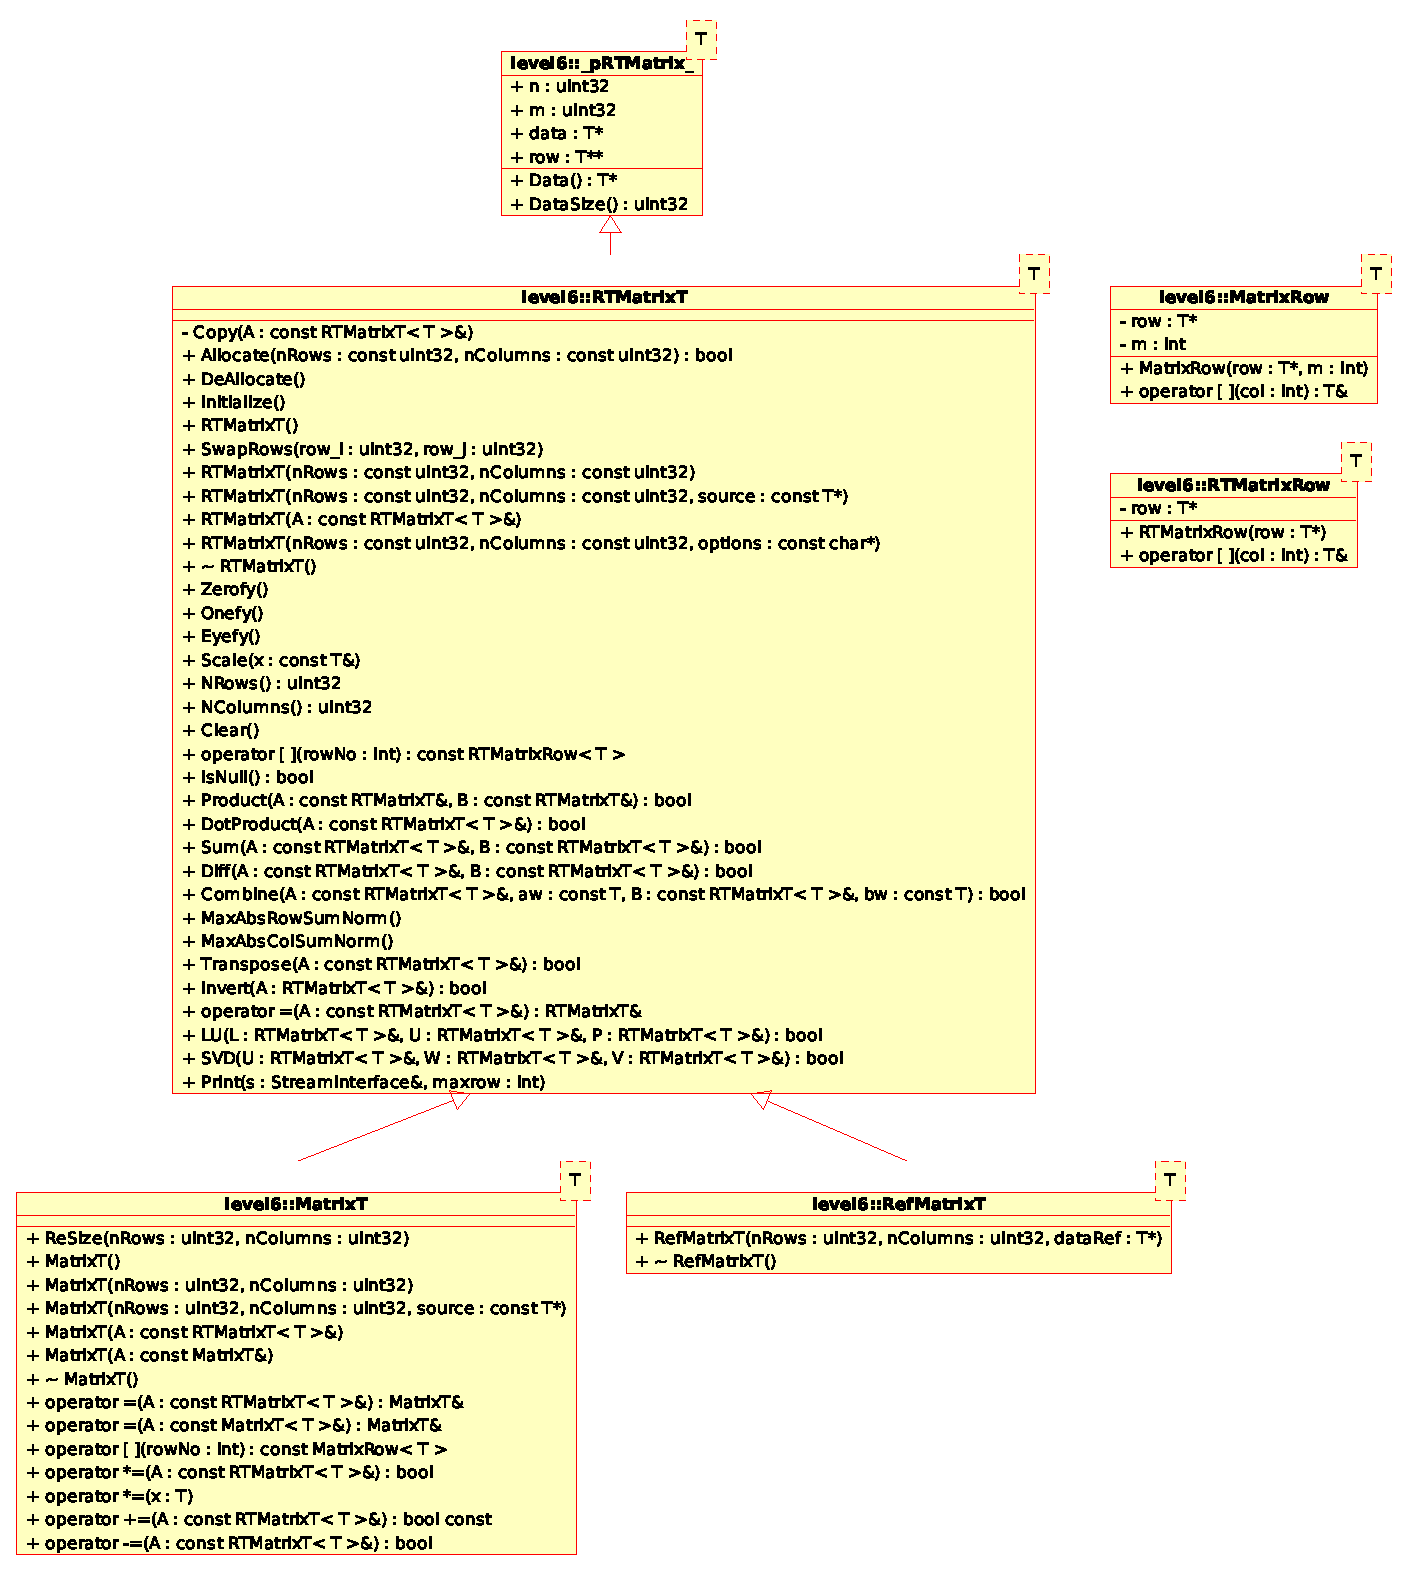
\includegraphics[width=0.88\textwidth]{level6/level6-math-matrix.eps}
  \caption{BaseLib Level 6 Mathematic Support Library}
  \label{f:level6:math-matrix}
 \end{center}
\end{figure}



\subsubsection{RTMatrixRow}
\texttt{[RTMatrix.h]}\\
The class \texttt{RTMatrixRow} is a class that holds a row of a generic matrix (in the source code its written that a \texttt{RTMatrixRow} is a orw of a \texttt{RTMatrix} but those classes have no links). As all classes in this section such class is templatized on the \texttt{T} parameter. The main attribute is a \texttt{T*} that holds a row of data, no other attributes are present.

To access the data in a simpler way the \texttt{\&operator[]} is redefined.

\begin{lstlisting}[
extendedchars=true,%
basicstyle=\fontfamily{pcr}\fontseries{m}\selectfont\footnotesize, %
stepnumber=1,%
numberstyle=\tiny,%
keywordstyle=\footnotesize\tt ,%
language=C++]
template <class T>
class RTMatrixRow{
   T* row;
public:
   inline RTMatrixRow(T *row);

   inline T &operator[](int col)const;
};
\end{lstlisting}



\subsubsection{MatrixRow}
\texttt{[Matrix.h]}\\
The class \texttt{MatrixRow} is anther implementation of a row of a matrix, this implementation is more rich. This class reimplement a row from scratch without inheriting from \texttt{RTMatrixRow}. It has not only the \texttt{T*} attribute but also an attribute \texttt{m} that count the number of elements in the row.

\begin{lstlisting}[
extendedchars=true,%
basicstyle=\fontfamily{pcr}\fontseries{m}\selectfont\footnotesize, %
stepnumber=1,%
numberstyle=\tiny,%
keywordstyle=\footnotesize\tt ,%
language=C++]
template <class T>
class MatrixRow{
   T* row;
   int m;
public:
   inline MatrixRow(T* row,int m);

   inline T &operator[](int col)const;
};
\end{lstlisting}



\subsubsection{\_pRTMatrix\_}
\texttt{[RTMatrix.h]}\\
The class \texttt{\_pRTMatrix\_} define the basic structure of a bidimensional matrix. It holds the main attributes to define a 2 dimensional matrix structure: the number of rows (\texttt{n} attribute) and the number of columns (\texttt{m} attribute); names of those attributes are not really explicit.

The attribute \texttt{data} is a pointer to the datas and \texttt{row} to the row information. The \texttt{data} attribute is returned by the \texttt{Data} method.
The method \texttt{DataSize} returns the number of elements in the matrix (row*columns).

\begin{lstlisting}[
extendedchars=true,%
basicstyle=\fontfamily{pcr}\fontseries{m}\selectfont\footnotesize, %
stepnumber=1,%
numberstyle=\tiny,%
keywordstyle=\footnotesize\tt ,%
language=C++]
template <class T>
class _pRTMatrix_ {
public:
   uint32 n;
   uint32 m;
   
   T *data;
   T **row;

   inline T *Data()const;
   inline uint32 DataSize()const;
};
\end{lstlisting}



\subsubsection{RTMatrixT}
\texttt{[RTMatrix.h, RTMatrix.cpp]} \\

The template class \texttt{RTMatrixT} is build upond the template class \texttt{\_pRTMatrix\_} and adds some important operations to matrix (bidimensional).

The method \texttt{Copy} copies or initialize an RTMatrix, it checks if the \texttt{data} pointer is NULL and in that case do the allocation.
The method \texttt{Initialize} initializes all the attributes to zero.

The first contructor simply calls \texttt{Initialize}, the second contructor calls \texttt{Allocate}; the third does the same but also load the datas. The fourth constructor calls \texttt{Copy}, the fifth constructor will be written for allocating a zeros, ones, eye matrix. The deconstructor simply call \texttt{Deallocate}.

\begin{lstlisting}[
extendedchars=true,%
basicstyle=\fontfamily{pcr}\fontseries{m}\selectfont\footnotesize, %
stepnumber=1,%
numberstyle=\tiny,%
keywordstyle=\footnotesize\tt ,%
language=C++]
template <class T>
class RTMatrixT:public _pRTMatrix_<T> {
private:
   void Copy(const RTMatrixT<T> &A);

public:
   bool Allocate(const uint32 nRows,const uint32 nColumns);
   void DeAllocate();

   void Initialize();

   inline void SwapRows(uint32 row_i, uint32 row_j);

   RTMatrixT();
   inline RTMatrixT(const uint32 nRows,const uint32 nColumns);
   inline RTMatrixT(const uint32 nRows,const uint32 nColumns,const T *source);
   inline RTMatrixT(const RTMatrixT<T> &A);
   inline RTMatrixT(const uint32 nRows,const uint32 nColumns,const char* options);
   inline ~RTMatrixT();
\end{lstlisting}

The method \texttt{Zerofy} sets elements of the matrix to zero; \texttt{Onefy} sets elements of the matrix to one; \texttt{Eyefy} sets the diagonal entries of the matrix to one, the others to zero.
The method \texttt{Scale} scales all the values by \texttt{x}.\\


The method \texttt{NRows} returns the number of rows of the matrix, \texttt{NColumns} returns the number of columns, \texttt{Clear} sets elements of the matrix to zero.
The method \texttt{IsNull} returns \texttt{True} if the matrix is the null one.

\begin{lstlisting}[
extendedchars=true,%
basicstyle=\fontfamily{pcr}\fontseries{m}\selectfont\footnotesize, %
stepnumber=1,%
numberstyle=\tiny,%
keywordstyle=\footnotesize\tt ,%
language=C++]
   inline void Zerofy();
   inline void Onefy();
   inline void Eyefy();
   inline void Scale(const T &x);

   inline uint32 NRows()const;
   inline uint32 NColumns()const;
   inline void Clear();

   inline const RTMatrixRow<T> operator[](int rowNo);

   inline bool IsNull();
\end{lstlisting}

Then follows a set of mathematical functions implemented in the class. The first method \texttt{Product} loads the product of matrix \texttt{A} and \texttt{B}. The method \texttt{DotProduct} is a product element by element. \texttt{Sum} loads the sum of matrix \texttt{A} and \texttt{B}. \texttt{Diff} loads the difference of matrix \texttt{A} and \texttt{B}.

The method \texttt{Combine} loads the linear combination of matrix \texttt{A} and \texttt{B}. Methods \texttt{MaxAbsRowSumNorm} and \texttt{MaxAbsColSumNorm} return the absolute maximum value of the rows or of the columns.

The method \texttt{Transpose} loads the transposed of \texttt{A}, \texttt{Invert} inverts the matrix \texttt{A} passed by reference. The assignement operator is then redefined to copy a matrix to another. \\


At the end follow the implementation of some really useful matrix operation the LUP decomposition (also called LU decomposition) and the SVD decomposition. The method \texttt{Print} just dumps on stream the matrix.

\begin{lstlisting}[
extendedchars=true,%
basicstyle=\fontfamily{pcr}\fontseries{m}\selectfont\footnotesize, %
stepnumber=1,%
numberstyle=\tiny,%
keywordstyle=\footnotesize\tt ,%
language=C++]
   inline bool Product(const RTMatrixT& A,const RTMatrixT& B);
   inline bool DotProduct(const RTMatrixT<T>& A)

   inline bool Sum(const RTMatrixT<T>& A,const RTMatrixT<T>& B);
   inline bool Diff(const RTMatrixT<T>& A,const RTMatrixT<T>& B);

   inline bool Combine(const RTMatrixT<T>& A,const T aw,const RTMatrixT<T>& B,const T bw);

   inline T MaxAbsRowSumNorm();
   inline T MaxAbsColSumNorm();

   inline bool Transpose(const RTMatrixT<T>& A);
   inline bool Invert(RTMatrixT<T>& A);

   inline RTMatrixT &operator=(const RTMatrixT<T>& A);

   bool LU(RTMatrixT<T>& L,RTMatrixT<T>& U,RTMatrixT<T>& P);
   bool SVD(RTMatrixT<T>& U,RTMatrixT<T>& W,RTMatrixT<T>& V);

   void Print(StreamInterface& s,int maxrow=10);
};
\end{lstlisting}



\subsubsection{MatrixT}
\texttt{[Matrix.h, Matrix.cpp]} \\
The class \texttt{MatrixT} is an extension of the class \texttt{RTMatrixT} with algebraic capabilities. It redefines the assignment operator, the access operator, the product, the sum and the difference operators.

\begin{lstlisting}[
extendedchars=true,%
basicstyle=\fontfamily{pcr}\fontseries{m}\selectfont\footnotesize, %
stepnumber=1,%
numberstyle=\tiny,%
keywordstyle=\footnotesize\tt ,%
language=C++]
template <class T>
class MatrixT: public RTMatrixT<T>{
public:
   void ReSize(uint32 nRows,uint32 nColumns);

   inline MatrixT();
   inline MatrixT(uint32 nRows,uint32 nColumns);
   inline MatrixT(uint32 nRows,uint32 nColumns,const T* source);
   inline MatrixT(const RTMatrixT<T>& A);
   inline MatrixT(const MatrixT& A);
   inline ~MatrixT();

   inline MatrixT &operator=(const RTMatrixT<T>& A);
   inline MatrixT &operator=(const MatrixT<T>& A);

   inline const MatrixRow<T> operator[](int rowNo);

   inline bool operator*=(const RTMatrixT<T>& A);
   inline void operator*=(T x);
   inline bool const operator+=(const RTMatrixT<T>& A);
   inline bool operator-=(const RTMatrixT<T>& A);
};
\end{lstlisting}



\subsubsection{RefMatrixT}
\texttt{[RefMatrix.h]} \\
The class template \texttt{RefMatrixT} create a matrix built on top of a C matrix, i.e. once created a C matrix you can manipulate it using a \texttt{RefMatrixT} and so all methods in \texttt{RTMatrixT}. Creating a new \texttt{RefMatrixT} from a C matrix you are being creating all the row pointers that speed up operations in the next phase of compuation.

\begin{lstlisting}[
extendedchars=true,%
basicstyle=\fontfamily{pcr}\fontseries{m}\selectfont\footnotesize, %
stepnumber=1,%
numberstyle=\tiny,%
keywordstyle=\footnotesize\tt ,%
language=C++]
template <class T>
class RefMatrixT: public RTMatrixT<T>{
public:
   RefMatrixT(uint32 nRows,uint32 nColumns,T* dataRef);
   ~RefMatrixT()
};
\end{lstlisting}



\subsection{Waveforms}
This section group togheter basically two class that let the user defining manually a waveform by defining touples of amplitude and time.

\begin{figure}[h!]
 \begin{center}
  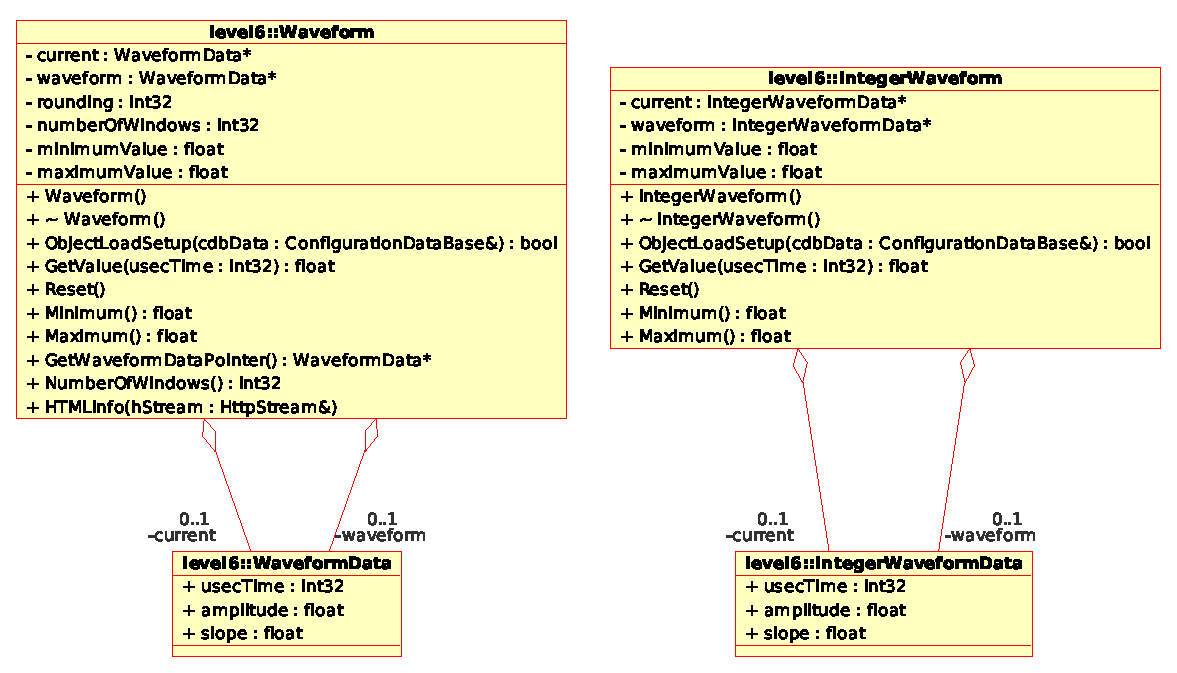
\includegraphics[width=0.88\textwidth]{level6/level6-math-waveform.eps}
  \caption{BaseLib Level 6 Mathematic Support Library}
  \label{f:level6:math-waveform}
 \end{center}
\end{figure}


Classes involved in this section are depicted in Figure \ref{f:level6:math-waveform} and listed below:

\begin{itemize}
 \item WaveformData, Waveform
 \item IntegerWaveformData, IntegerWaveform
\end{itemize}


\subsubsection{WaveformData, Waveform}
\texttt{[Waveform.h]}\\
The class \texttt{Waveform} lets the user define a specified waveform of data. The basic data structure of a waveform is the \texttt{WaveformData} structure that holds each amplitude and time of the defined signal.

\begin{lstlisting}[
extendedchars=true,%
basicstyle=\fontfamily{pcr}\fontseries{m}\selectfont\footnotesize, %
stepnumber=1,%
numberstyle=\tiny,%
keywordstyle=\footnotesize\tt ,%
language=C++]
struct WaveformData {
   int32 usecTime;
   float amplitude;
   float slope;
};
\end{lstlisting}

The class \texttt{Waveform} keeps its internal time in microseconds but loads data from CDB in seconds. Note that all \texttt{slope}s are calculated at the moment of creation (during methods \texttt{ObjectLoadSetup}), and that the waveform has to be resetted (function \texttt{Reset}) between a pulse and the other. \\


The first attribute, \texttt{current} is a pointer to the current element in the \texttt{Waveform}, \texttt{waveform} is a pointer to the first element in the \texttt{Waveform} array.

The attribute \texttt{rounding} is a rounding factor for conversion between seconds and microseconds, \texttt{numberOfWindows} is the number of time windows. The attribute \texttt{minimumValue} and \texttt{maximumValue} are respectively the minimum and the maximium value of the waveform.

\begin{lstlisting}[
extendedchars=true,%
basicstyle=\fontfamily{pcr}\fontseries{m}\selectfont\footnotesize, %
stepnumber=1,%
numberstyle=\tiny,%
keywordstyle=\footnotesize\tt ,%
language=C++]
class Waveform {
private:
   WaveformData* current;
   WaveformData* waveform;
   int32 rounding;
   int32 numberOfWindows;

   float minimumValue;
   float maximumValue;
\end{lstlisting}

Using method \texttt{ObjectLoadSetup} its possible to load a \texttt{Waveform} from a CDB; in this case you have to define in the configuration file two arrays: \texttt{Times} and \texttt{Amplitudes}.
The method \texttt{GetValue} returns the value of the waveform at a certain time. The method \texttt{Reset} resets the internal states and waveforms; to be called in the ``PREPULSE'' phase. \texttt{Minimum} returns waveform's minimum value; \texttt{Maximum} returns waveform's maximum value. \texttt{GetWaveformDataPointer} returns \texttt{waveform} attribute value. \texttt{NumberOfWindows} gets number of windows in the current waveform. \texttt{HTMLInfo} print the information about the waveform with HTML format.

\begin{lstlisting}[
extendedchars=true,%
basicstyle=\fontfamily{pcr}\fontseries{m}\selectfont\footnotesize, %
stepnumber=1,%
numberstyle=\tiny,%
keywordstyle=\footnotesize\tt ,%
language=C++]
public:
   Waveform();
   virtual ~Waveform();

   bool ObjectLoadSetup(ConfigurationDataBase& cdbData);

   inline float GetValue(int32 usecTime);

   inline void Reset();

   float Minimum();
   float Maximum();
   inline WaveformData* GetWaveformDataPointer();
   inline int32 NumberOfWindows();

   void HTMLInfo(HttpStream& hStream);
};
\end{lstlisting}



\subsubsection{IntegerWaveformData, IntegerWaveform}
\texttt{[IntegerWaveform.h]}\\
The class \texttt{IntegerWaveform} works thanks to an \texttt{IntegerWaveformData} structure. Such structure holds data for a single element in an \texttt{IntegerWaveform}.
The class is the same as the class \texttt{WaveformData}.

\begin{lstlisting}[
extendedchars=true,%
basicstyle=\fontfamily{pcr}\fontseries{m}\selectfont\footnotesize, %
stepnumber=1,%
numberstyle=\tiny,%
keywordstyle=\footnotesize\tt ,%
language=C++]
struct IntegerWaveformData {
   int32 usecTime;
   float amplitude;
   float slope;
};
\end{lstlisting}

An \texttt{IntegerWaveform} is similar to a \texttt{Waveform} and keeps its internal time in microseconds; in the same way all slopes are calculated at the moment of creation (during function \texttt{ObjectLoadSetup}). Attributes have also the same meaning.

\begin{lstlisting}[
extendedchars=true,%
basicstyle=\fontfamily{pcr}\fontseries{m}\selectfont\footnotesize, %
stepnumber=1,%
numberstyle=\tiny,%
keywordstyle=\footnotesize\tt ,%
language=C++]
class IntegerWaveform {
private:
   IntegerWaveformData* current;
   IntegerWaveformData* waveform;
   
   float minimumValue;
   float maximumValue;

public:
   IntegerWaveform();
   virtual ~IntegerWaveform();

   bool ObjectLoadSetup(ConfigurationDataBase& cdbData);
   inline float GetValue(int32 usecTime);

   inline void Reset();

   float Minimum();
   float Maximum();
};
\end{lstlisting}



\subsection{Filters}

TODO

\subsubsection{Filter}
\texttt{[Filter.h, Filter.cpp]}\\
The class \texttt{Filter} implements a single input single output filter. Initialisation is performed via CDB, i.e. it must be written in the configuration file. The class descend only from \texttt{Object}.

A filter in the configuration file can be defined in different ways as the table below explains:


\begin{table}[!h]
 \begin{center}
  \begin{tabular}{|l|c|}
   \hline
Numerator  = \{a0 a1 a2...\} & \\
Denominator= \{b0 b1 .... \} & \\
   \hline
0  = \{a0 a1 a2...\} & b0 assumed to be 1 \\
1  = \{-b1 -b2.... \} & \\
   \hline
Poles  = \{p0 p1 ... \} & $\frac{p0}{S + p0} * \frac{p1}{S + p1}$  \\
Zeros  = \{z0 z1 ... \} & $\frac{S + z0}{z0} * \frac{S + z1}{z1}$  \\
SamplingTime = 1e-3 & \\
Gain = g  & which multiplies the whole expression \\
   \hline
  \end{tabular}
 \end{center}
\end{table}

The first two filter configuration are already expressed in z domain, the last one is expressed in s domain and the Filter class discretizes the transfer function using Tustin bilinear transformation.

\begin{lstlisting}[
extendedchars=true,%
basicstyle=\fontfamily{pcr}\fontseries{m}\selectfont\footnotesize, %
stepnumber=1,%
numberstyle=\tiny,%
keywordstyle=\footnotesize\tt ,%
language=C++]
private:
   int inputSize;
   int outputSize;

   float* inputStatus;
   float* outputStatus;
   double* inputCoefficients;
   double* outputCoefficients;

private:
   bool InitP(ConfigurationDataBase &cdb);
   bool Resize(int inputSize,int outputSize);

public:
   ~Filter();
   Filter();

   bool Init(ConfigurationDataBase &cdb);
   inline void Reset(float input=0.0,float output=0.0);

   inline float Process(float input);
\end{lstlisting}



\subsection{Coords}
TODO



\section{HTTP Browsing}

TODO

\begin{figure}[h!]
 \begin{center}
  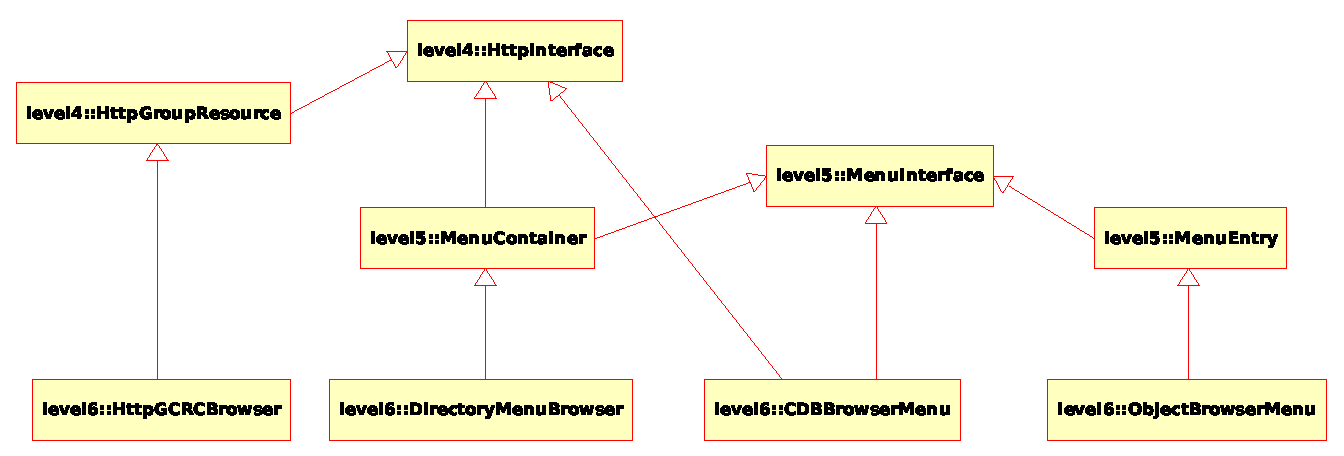
\includegraphics[width=\textwidth]{level6/level6-Browser.eps}
  \caption{BaseLib Level 6 HTTP Browsing}
  \label{f:level6:HTTPbrowser}
 \end{center}
\end{figure}



\section{System Support}

TODO

\begin{figure}[h!]
 \begin{center}
  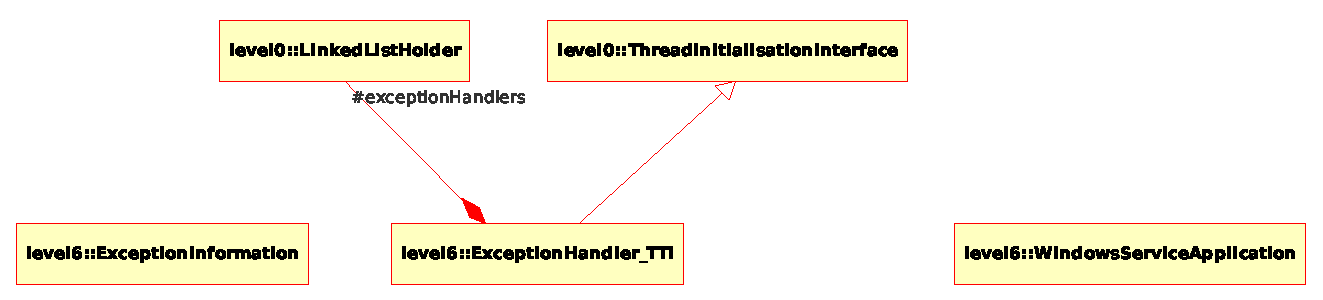
\includegraphics[width=\textwidth]{level6/level6-system.eps}
  \caption{BaseLib Level 6 System Support Library}
  \label{f:level6:system}
 \end{center}
\end{figure}



\subsection{Design Notes}
System support must be moved to level0.
